
%%%%%%%%%%%%%%%%%%%%%%%%%%%%----->SECCIÓN 3<-----%%%%%%%%%%%%%%%%%%%%%%%%%
\newpage
\chapter{Modulación del fondo de Rayos Cósmicos debido a la actividad Solar}

%%%%%%%%%%%%%%%%%%%%%%%%%%%%% NEWW
En este capítulo, presentaremos los resultados obtenidos del estudio de la modulación de los Rayos Cósmicos Galácticos (GCR) debido a la actividad solar, utilizando el Observatorio Pierre Auger. Aquí, nos encofaremos en examinar la sensibilidad del Observatorio Pierre Auger a las fluctuaciones en la actividad solar a corto y largo plazo.

Como se describió en el capítulo 1, la interacción entre los GCR y el viento solar provoca cambios en la cantidad de GCR detectados. El viento solar, que se ve afectado por fenómenos periódicos como la rotación solar de \~27 días, el ciclo de 11 años que está asociado a emisiones de plasma desde la corona y a un cambio en la frecuencia de las eyecciones de masa coronal (CME) (\cite{belov_2021} entre otros).

Los estudios previos realizados en el Observatorio han demostrado que el modo Scaler es altamente sensible a las condiciones del medio interplanetario determinadas por la actividad solar (\cite{Martin_Schimassek2022}). Esta sensibilidad permite que los datos recopilados en el modo Scaler proporcionen información complementaria a la obtenida a través de los monitores de neutrones, abriendo una ventana energética diferente a los rayos cósmicos de baja energía.

Comenzaremos con una descripción de los datos y las fuentes que hemos utilizado para este estudio, seguido de una explicación de cómo se procesaron los datos en modo Scaler del arreglo de detectores para garantizar la fiabilidad. A continuación, realizaremos una comparación entre las mediciones realizadas por Detectores de Neutrones y las obtenidas en el Observatorio Pierre Auger, destacando las ventajas y desventajas de cada uno en el contexto de nuestro estudio. Finalmente, discutiremos los efectos de la actividad solar en el fondo de rayos cósmicos a corto y largo plazo, proporcionando una visión completa de cómo la actividad solar puede influir en la detección de GCR.

\section{Datos}

En este trabajo, se utilizaron las siguientes bases de datos :
\begin{enumerate}

\item Scalers del Observatorio Pierre Auger: Se utilizaron datos de intensidad de rayos cósmicos del Observatorio Pierre Auger, corregidos por presión y temperatura utilizando el software \textit{ScalerAnalysis}\footnote{\url{https://opendata.auger.org/}}.
    \item Datos de detectores de neutrones: Se utilizaron datos de intensidad de rayos cósmicos de varias estaciones, incluyendo Oulu\footnote{\href{https://cosmicrays.oulu.fi/}{Cosmic Ray Station}  of the University of Oulu / Sodankyla Geophysical Observatory 
}, Athenas, México, y Tsumeb. Estos datos, con una resolución de 3 horas, fueron corregidos por presión y temperatura \footnote{Agradecemos el suministro de datos a la base de datos NMDB (www.nmdb.eu), creada en el marco del programa FP7 de la Unión Europea (contrato nº 213007).  \url{//www.nmdb.eu/nest/}}.
    \item Datos del viento solar: Se obtuvieron datos del viento solar del Space Physics Data Facility (SPDF) de la NASA \footnote{\url{https://spdf.gsfc.nasa.gov/pub/000_readme.htm}}.
    \item Datos de manchas solares: Se utilizaron datos de manchas solares del Centro de Datos Mundial SILSO, Real Observatorio de Bélgica, Bruselas (Sunspot Index and Long-term Solar Observations)(\cite{sidc})\footnote{\url{https://www.sidc.be/SILSO/datafiles}} . Es una parte del SIDC (Solar Influences Data Analysis Center), que es el departamento de física solar del Real Observatorio de Bélgica. SILSO se dedica a la producción, preservación y difusión del número internacional de manchas solares.
    \item Base de datos de Forbush Decreases: Se usó el Catálogo de los efectos Forbush y de las perturbaciones interplanetarias, creada por el Instituto Pushkov de Magnetismo Terrestre, Ionosfera y Propagación de Ondas de Radio de la Academia de Ciencias de Rusia (IZMIRAN). Esta base de datos es la única disponible que es integral y actualizada sobre los efectos de Forbush (\cite{okike_2021})\footnote{Instituto Pushkov de Magnetismo Terrestre, Ionosfera y Propagación de Ondas de Radio de la Academia de Ciencias de Rusia (IZMIRAN). (1957-2019). Izmiran Catalogue of the Forbush-effects and interplanetary disturbances (Versión 2021-04-16) [Eventos Forbush] \url{http://spaceweather.izmiran.ru/eng/dbs.html}.}.
\end{enumerate}

\begin{table}[ht]
\centering
\caption{Caption}
\small
\begin{tabular}{ccccccc}
\toprule
\textbf{Detector} & \textbf{Latitud} & \textbf{Longitud} & \textbf{Rigidez de corte} & \textbf{Altitud (msmm)} & \textbf{Tipo} & \textbf{Hora local} \\
\midrule
NM Oulu & \ang{65.05}N & \ang{25.46}E & 0.8GV & 15M & 9-NM64 & UTC+2 \\
NM Athenas & \ang{37.97}N & \ang{23.78}E & 8.53GV & 260m & 6-NM64 & UTC+2 \\
NM Tsumeb & \ang{19.12}S & \ang{17.35}E & 9.2GV & 1240M & 18-NM64 & UTC+2 \\
NM México & \ang{19.33}N & \ang{99.18}W & 8.2GV & 2274m & 6-nm64 & UTC-6 \\
SD Pierre Auger& \ang{35.3}S & \ang{69.3}O & 9.5GV & 1400m & Muones & UTC-3 \\
\bottomrule
\end{tabular}
\label{tab:my_label}
\end{table}


\section{Procesamiento de datos en modo Scaler}

El estudio de los scalers puede involucrar períodos de horas hasta varios años, lo cual exige el establecimiento de criterios para el procesamiento de datos más detallado que tenga en cuenta las inestabilidades del arreglo de superficie por el gran número de detectores, y las variaciones en las condiciones atmosféricas. Con el fin de mejorar la calidad de los datos para los estudios de física solar, se han implementado correcciones y selecciones que aseguran la confiabilidad del conjunto de datos, demostrando su aptitud para el análisis de fenómenos solares mediante la identificación de señales conocidas y previstas en distintos intervalos de tiempo.

Trabajos anteriores dentro de la colaboración ( \cite{bertou_2011}  \cite{asorey} \cite{masias_2017} \cite{Martin_Schimassek2022}), se han enfocado en refinar las metodologías y criterios estadísticos que permitan un procesamiento adecuado manteniendo la integridad de la información física que subyace a cada una de las detecciones del arreglo. A la fecha, se cuenta con un framework robusto para el procesamiento que garantiza la uniformidad en los dataset utilizados para cualquier intervalo de tiempo en donde el arreglo de superficie esté en funcionamiento: \textit{Scaler Analysis}  (\cite{martin_ICRC}). A continuación veremos de forma más detallada cómo se implementan las correcciones en el framework .

El primer criterio fundamental es efectuar todas las correcciones a nivel de estación individual para potenciar la extracción de datos. Para asegurar la integridad de los datos, nos basamos en la información del estado de los PMT, que se obtiene del análisis de las trazas de las lluvias de aire, y seleccionamos de manera selectiva las estaciones que cuentan con tres PMT operativos. Este método de selección actualizado reemplaza los antiguos cortes que se realizaban en el tratamiento de datos que solo realizaban cortes en la distribución total de la tasa de scaler \cite{martin_ICRC}.

La información necesaria para el procesamiento de los scaler (1 dato/s) no se encuentra en un solo conjunto de datos y no comparten el mismo intervalo de muestreo. Se requiere información del monitoreo del detector (300s), detalles sobre el estado del PMT disponibles en los datos de eventos (1 día), e información sobre las condiciones atmosféricas y meteorológicas (300s). Para combinar de manera efectiva toda esta información, el software utilizado en este trabajo se basa en la idea de que la recopilación y fusión de datos puede separarse del análisis en sí mismo. Gracias a esta separación, el análisis se organiza en “módulos” que pueden ser específicos para el análisis, manteniendo ocultos los detalles del tratamiento de la información de entrada. Finalmente, se crea un dataset depurado que incluye los promedios de la tasa de scaler en un intervalo de tiempo personalizado. Para este trabajo hemos adoptado un intervalo de cinco minutos. En la Figura \ref{esquema_datos}, se muestra un esquema del flujo de datos utilizado en el \textit{Scaler Analysis}. 

En síntesis, las correcciones se plantean secuencialmente de la siguiente manera:

\begin{figure}
\centering
    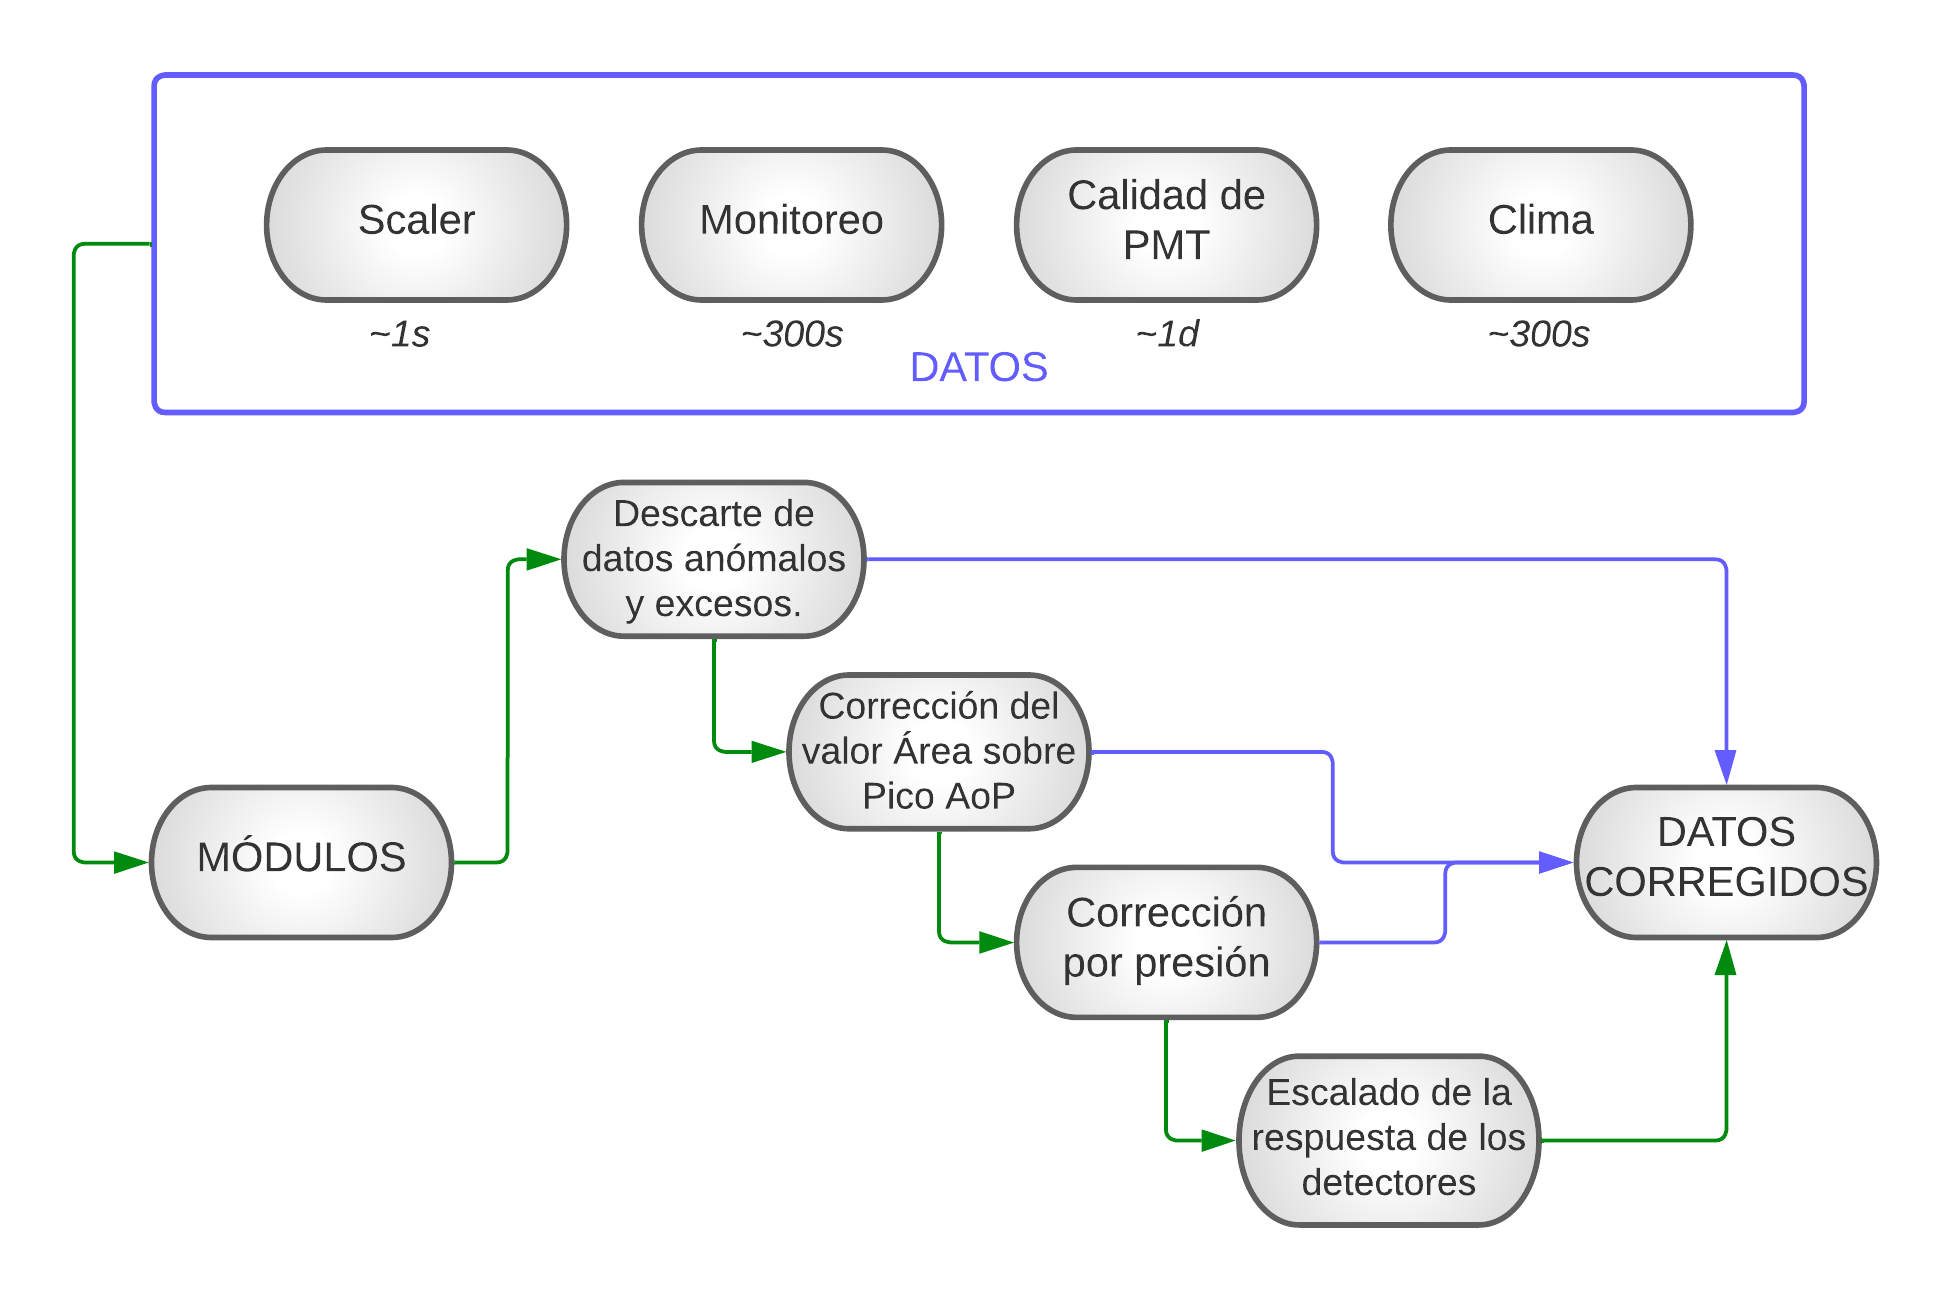
\includegraphics[width=0.7\linewidth]{Figs/SCALER.png}
    \caption{Enter Caption}
    \label{esquema_datos}
\end{figure}
\textbf{Identificación de estaciones erróneas:} Para asegurar la calidad de los datos, solo se seleccionan las estaciones que están configuradas para recoger y transmitir datos válidos cada segundo conforme a los siguientes criterios:
\begin{enumerate}
    \item Estaciones donde los 3 PMT estén en funcionamiento.
    \item Una relación área sobre pico entre $2.5 < AoP < 4.5$ para excluir estaciones que están muy fuera del rango de trabajo normal.
    \item   Estaciones con todos los PMT cumpliendo que $35 < I_{peak}/FADC < 65$. El rango corresponde a una desviación de $\pm30\%$ del valor de diseño tratando de mantener tantas estaciones como sea posible en el análisis.
    \item Se descartan estaciones de las que no se tenga señal de monitoreo.
\end{enumerate}

\textbf{Estaciones atípicas:} Se eliminan las estaciones que notifican tasas de recuento excepcionalmente altas en un solo segundo. Para detectar estos valores atípicos, se utiliza la Desviación Absoluta Mediana (MAD, por sus siglas en inglés). La MAD es una medida de la variabilidad de un conjunto de datos y se define como la mediana de las desviaciones absolutas de los datos con respecto a su mediana. Entonces para cada punto de datos, se calcula cuánto se desvía la mediana del conjunto de datos, se toma el valor absoluto de esa desviación, y luego se obtiene la mediana de todas esas desviaciones. Para cada segundo en la estación, se calcula el valor $z$ que es una medida de cuántas desviaciones estándar puede un dato estar lejos de la media:
\begin{equation}
    z=\frac{\Gamma-\tilde{\Gamma}}{\tilde{\sigma}}
\end{equation}

Donde $\tilde{\Gamma}$ es la mediana y $\tilde{\sigma}$ es la desviación absoluta mediana.  Si  $z>3$ la estación y el segundo se marcan como valores atípicos. En este caso, en lugar de utilizar la media y la desviación estándar, se utilizan la mediana y la MAD, lo que hace que esta medida sea más resistente a los valores atípicos.

\textbf{Rayos y excesos localizados:} Debido al bajo umbral del Scaler, los datos son sensibles a los impulsos electromagnéticos de los rayos, lo que es crucial para el rechazo del ruido de fondo. Se utiliza un método similar a la búsqueda de aumentos de tasa correlacionados con estallidos de rayos gamma para identificar segundos con impactos de rayos. El uso de intervalos de cinco minutos permite una sólida estimación de las tasas medias. Además, un modelo de fondo gaussiano con una señal adicional común facilita la evaluación del exceso de significación, ayudando a marcar los valores atípicos.

\textbf{Promedio y escala:} Se calcula la media aritmética de todos los segundos de cada estación, excluyendo los eliminados por criterios previos. Luego, se obtiene la media de todas las estaciones, enfocándose en el análisis de una sola estación. Esta elección mantiene la claridad conceptual, ya que las correcciones de los efectos a largo plazo se aplican por estación. No se utiliza ninguna ponderación con el número de segundos activos, lo que garantiza la distinción numérica del promedio sobre estaciones por segundo. Para estas correcciones, se utilizan cantidades promediadas como la presión atmosférica y el Área sobre Pico.

\textbf{Correcciones por tendencias a largo plazo:} 

Las tendencias a largo plazo, debidas al envejecimiento de los detectores y a los cambios atmosféricos, requieren correcciones que incluyen: 
\begin{itemize}
    \item Fluctuaciones en la presión atmosférica que corrijan la anticorrelación esperada con la tasa de scaler, esto se puede ajustar con un modelo lineal simple:
\begin{equation}
    \Gamma_{corrected}(t)=\Gamma(t)-a_{1}(p(t)-\langle p\rangle)
\end{equation}
    \item Corrección de área sobre pico (AoP) que se realiza para ajustar los cambios en la forma del pulso en el Detector de Superficie (SD) a lo largo del tiempo. Este ajuste es esencial para estudios a largo plazo, ya que el AoP cambia en una escala de años. El modelo para esta corrección se basa en dos premisas: la señal total disponible (es decir, el número de fotones) en el tanque escala con la calidad óptica del revestimiento acuoso, y la probabilidad de activar todos los tres PMT con una señal de baja energía también escala con la reflectividad del revestimiento. Así, el número esperado de fotoelectrones en el tiempo estaría dado por:
\begin{equation}
    n_{ph}\approx \int s_{ADC}(t|n_{0})  dt  \propto AoP n_{0}
\end{equation}

Donde $s_{ADC}(t|n_{0})$ es la señal integrada en el tiempo en función del número de fotones Cherenkov creados $n_{0}$. 

    \item  Corrección de la línea de base que es el ajuste que se debe realizar para tener en cuenta los cambios constantes en las mediciones de los tubos fotomultiplicadores (PMT), que están correlacionados con la temperatura. Debido a la naturaleza entera de los convertidores analógico-digitales (FADC), y por lo tanto los umbrales del Scaler, esto puede llevar a cambios residuales en la tasa medida.
\end{itemize} 

\section{Detectores de Neutrones vs Pierre Auger}

%(Hatton & Carimichael, 1964)
Los monitores de neutrones (NMs) son una herramienta esencial utilizada en todo el mundo para medir el flujo de partículas secundarias que llegan a la Tierra. Estos detectores terrestres están diseñados para registrar neutrones secundarios generados en lluvias atmosféricas provocadas por iones de rayos cósmicos. Aunque el NM fue inventado por John Simpson en 1958, el diseño estándar que se utiliza actualmente se desarrolló en 1964 (NM64), y se ha convertido en un detector estándar de rayos cósmicos terrestres (\cite{eleana_2017}).

Desde su invención, se ha establecido una extensa red global de estos instrumentos, que abarca desde varias decenas hasta un máximo de 70 estaciones distribuidas en todo el mundo. Los datos recopilados por esta red se utilizan para evaluar las variaciones en el flujo de rayos cósmicos galácticos en el rango de energía de 1 a 100 GeV, proporcionando información crucial sobre el impacto de las tormentas solares, las eyecciones de masa coronal, las estructuras del viento solar y el ciclo de actividad solar en la modulación de los rayos cósmicos (\cite{Ruffolo_2016}).

Los NMs tienen la propiedad de que su dirección de observación barre el espacio con la rotación de la Tierra, por lo que las variaciones diarias (diurnas) en la tasa de recuento de NM proporcionan información adicional sobre la distribución direccional y la anisotropía de los rayos cósmicos (\cite{Ruffolo_2016}). Estos instrumentos utilizan materiales propensos a reacciones nucleares con neutrones, como el litio o el boro.

Debido a que los neutrones son partículas sin carga eléctrica, estos instrumentos se valen de las interacciones posibles de los neutrones energéticos con los núcleos atómicos: colisiones elásticas e inelásticas y reacciones nucleares para producir neutrones rápidos que luego son frenados por un material hidrogenado y medidos indirectamente a través de las partículas ionizantes producidas.

La figura \ref{fig:NM_schem} muestra un diagrama esquemático del monitor de neutrones 6-NM64 ubicado en Atenas, Grecia. El número 6 indica el número de tubos contadores con los que cuenta la estación. La parte b muestra la estructura interna de este detector, en la que se pueden identificar 4 componentes principales: El tubo contador que contiene principalmente $BF_{3}$ (trifluoruro de boro) que al interactuar con los neutrones térmicos producen iones de litio y partículas alfa que al ser acelerados ionizan el gas y producen electrones que provocan una señal que puede ser medida y procesada. Los tubos contadores están recubiertos por una capa moderadora que consta de un tubo de polietileno de 2 cm de espesor que absorbe y refleja los neutrones de evaporación que son generados en el productor de plomo. La capa productora que funciona como blanco de elevada masa atómica, en este caso es plomo, para producir neutrones secundarios y finalmente otra capa reflectora de polietileno (\cite{OlgaMalandraki_2018}).


\begin{figure}
\centering
    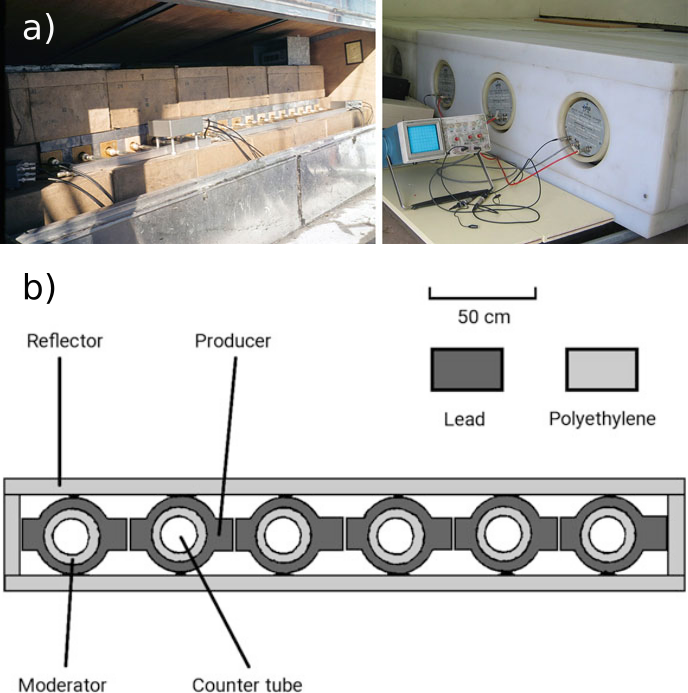
\includegraphics[width=0.7\linewidth]{Figs/NM_schem.png}
    \caption[Diagrama esquemático del monitor de neutrones 6-NM64 ubicado en Atenas, Grecia.]{Diagrama esquemático del monitor de neutrones 6-NM64 ubicado en Atenas, Grecia. El número 6 indica el número de tubos contadores con los que cuenta la estación. La parte b muestra la estructura interna de este detector, en la que se pueden identificar 4 componentes principales: El tubo contador que contiene principalmente $BF_{3}$ (trifluoruro de boro) que al interactuar con los neutrones térmicos producen iones de litio y partículas alfa que al ser acelerados ionizan el gas y producen electrones que provocan una señal que puede ser medida y procesada. Los tubos contadores están recubiertos por una capa moderadora que consta de un tubo de polietileno de 2 cm de espesor que absorbe y refleja los neutrones de evaporación que son generados en el productor de plomo. La capa productora que funciona como blanco de elevada masa atómica, en este caso es plomo, para producir neutrones secundarios y finalmente otra capa reflectora de polietileno. Fuente: \cite{OlgaMalandraki_2018}}
    \label{fig:NM_schem}
\end{figure}
%%%%%%%%%%% BOOOK  Solar Particle Radiation Storms Forecasting and Analysis

%%%%%%%%%%%%%%%%%%%%%%%%%%%
%%%MEJORA REDACCIÓNNNNNN
\begin{comment}
A rasgos generales la tasa de recuento total puede presentarse como una suma de tasas de recuento $N_{i}$ debidas a diferentes especies de GCR:

\begin{equation}
    N = \sum_{i}N_{i} = \sum_{i}\int_{Tci}^\infty J_{i}(T, \phi)Y_{i}(T)dT
\end{equation}
%%%MEJORA REDACCIÓNNNNNN::::
donde Y i es la función de rendimiento específico de NM para la ith especie de GCR, y la integración es sobre la energía cinética por encima de T ci, que es la energía cinética correspondiente a la corte de rigidez geomagnética local Pc y es diferente para diferentes especies de rayos cósmicos. Aquí sólo consideramos las dos especies de RC más abundantes, los protones y las partículas a. Puesto que la contribución de las especies más pesadas es pequeña y su modulación es similar a la de las partículas helio. modulación es similar a la del helio, no las consideramos aquí. aquí. Mientras que la fracción de partículas a es de alrededor del 20$\%$ (en número de nucleones) en LIS, su contribución a la tasa de recuento de NM varía del 23$\%$(NM polar, mínimo solar) al 37$\%$ (NM ecuatorial, máximo solar). (NM ecuatorial, máximo solar) (\cite{Usoskin_2005}).
\end{comment}

Se ha mostrado que el observatorio Pierre Auger funciona también como sensor de las fluctuaciones de los rayos cósmicos galácticos GCR. Sin embargo, como se describió en el capítulo 1, además de las influencias del espacio exterior, la intensidad de los rayos cósmicos observados a nivel del suelo también está determinada por el campo magnético y la atmósfera de la Tierra.  El campo geomagnético desvía las trayectorias de los rayos cósmicos en función de su rigidez de corte, adquiriendo una distribución dependiendo de la ubicación geográfica (\cite{herbst_2013influence}). Esto se traduce en diferencias en las señales medidas por cada una de las estaciones ubicadas alrededor del mundo. 

En la figura \ref{NM_compar} se observa la intensidad de rayos cósmicos normalizada medida para las estaciones de neutrones de Oulu, México, Athenas, Tsumeb comparadas con la tasa de scaler. En la gráfica se observa el comportamiento desde el 2006 hasta el 2021, en donde tenemos todo el ciclo solar 24 (2008-2019). Se observa que todas las estaciones incluido Auger presentan un aumento en el flujo durante los periodos de menor actividad solar y un decremento en la zona de mayor actividad. Observamos también que las estaciones con mayor rigidez de corte presentan una menor variabilidad, sin embargo, la señal del Observatorio Pierre Auger parece estar mucho más atenuada. Indagaremos esto, estimando la sensibilidad que tiene el observatorio ante la actividad solar de corto y largo plazo.
\begin{figure}
\centering
    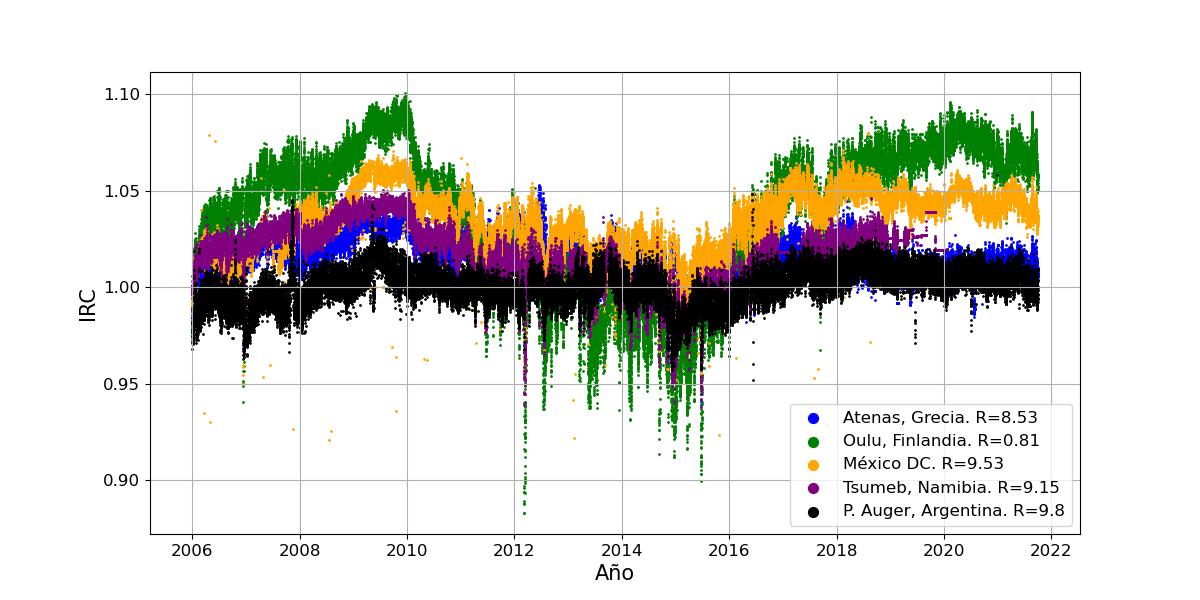
\includegraphics[width=1.1\linewidth]{Figs/Figr/NM_Auger_comparison.png}
    \caption[Diagrama esquemático del monitor de neutrones 6-NM64 ubicado en Atenas, Grecia.]{Intensidad de rayos cósmicos normalizada medida para las estaciones de neutrones de Oulu, México, Athenas, Tsumeb comparadas con la tasa de scaler. En la gráfica se observa el comportamiento desde el 2006 hasta el 2021, en donde tenemos todo el ciclo solar 24 (2008-2019). Se observa que todas las estaciones incluido Auger presentan un aumento en el flujo durante los periodos de menor actividad solar y un decremento en la zona de mayor actividad.  . Elaboración propia}
    \label{NM_compar}
\end{figure}

%%%%%%%%%%%%%%%%%%%%%%%%%%%%%%%%%%%%%%%%%%%%
% TRABAJO CON LOS DATOSSSSSSSSSSSSSSSSSSSSSSSS
Esta comparación se ha realizado considerando que cada dataset, aún corregido puede presentar valores anómalos relacionados a fallas en la detección y inconsistencias en los parámetros de calibración (menos del $1\%$ de los datos). Por esta razón, se aplicó el método de interpolación e imputación para completar los datos faltantes o nulos y generar un series de tiempo consistentes (\cite{wang_2019}).
%%%%%%%%%%%%%%%%%%%%%%%%%%%%%%%%%%%%%
%
%Mediante la figura (xxxx) podems observar perfiles construidos a partir de la técnica de época superpuesta para diferentes observables: La ICME-sheath se muestra con fondo color naranja (intervalo 0 < t < 1), y la ICME con fondo azul (1 < t < 4). El dominio temporal t está normalizado con la duración de la sheath para t < 1, y con la duración de la ICME para t > 1 (la ICME esta representada de tal forma que dura 3 veces más que la sheath, para asemejarse a los casos individuales). Los puntos negros son valores medios para cada bin temporal, los puntos rojos son las medianas asociadas. %%% COLOCAR PIE DE PÁGINA CON LAS EXPLICACIONES MAYBE


\section{Modulación de GCR medido en el Observatorio Pierre Auger}
%%%%%%%%%%%NEWWW
%Verificar cómo hablo de las ICME en el capítulo 1
Una ICME (Eyección de Masa Coronal Interplanetaria) es una gran expulsión de plasma y campo magnético del Sol que se propaga a través del espacio interplanetario. Estas ICMEs pueden influir significativamente en el transporte de los Rayos Cósmicos Galácticos (GCRs) y tienen efectos tanto a nivel local como global en la densidad de GCRs (\cite{Davies_2023}). Estos efectos están relacionados con cambios significativos en las características locales de la turbulencia en el medio interplanetario, así como la presencia de estructuras con líneas de campo magnético suaves e intensas en las nubes que alteran la configuración del viento solar (\cite{Krittinatham_2009}) (Ver capítulo 1).

La Figura \ref{fig:ICME_scaler} realizada en un trabajo previo por \cite{masias_2017}, muestra los perfiles superpuestos de los flujos de GCR para diferentes energías en el Observatorio Pierre Auger durante el paso de una ICME. Se observa un aumento en la magnitud del campo magnético interplanetario B, y las fluctuaciones magnéticas rmsB alcanzan su valor máximo en el choque. Las gráficas muestran las desviaciones normalizadas del flujo de scaler, y las dos bandas de histograma. En los datos de scaler se observa una disminución de hasta el −0.3\% a la que le sigue una recuperación similar al efecto observado con los detectores de neutrones. Estos mismos efectos son observados con los modos histograma $H_{sc}$ y $H_{\mu}$ con diferente intensidad llegando a ser hasta de −0.4\%.

Así, durante los periodos de alta actividad solar donde las ICMEs son más frecuentes, van a causar variaciones significativas en los datos del observatorio. Por otro lado, durante los periodos de baja actividad solar, las ICMEs al ser menos frecuentes, mantendrá más estable los datos del observatorio.

%%%%%%%%%%% NEWWW


\begin{figure}
\centering
    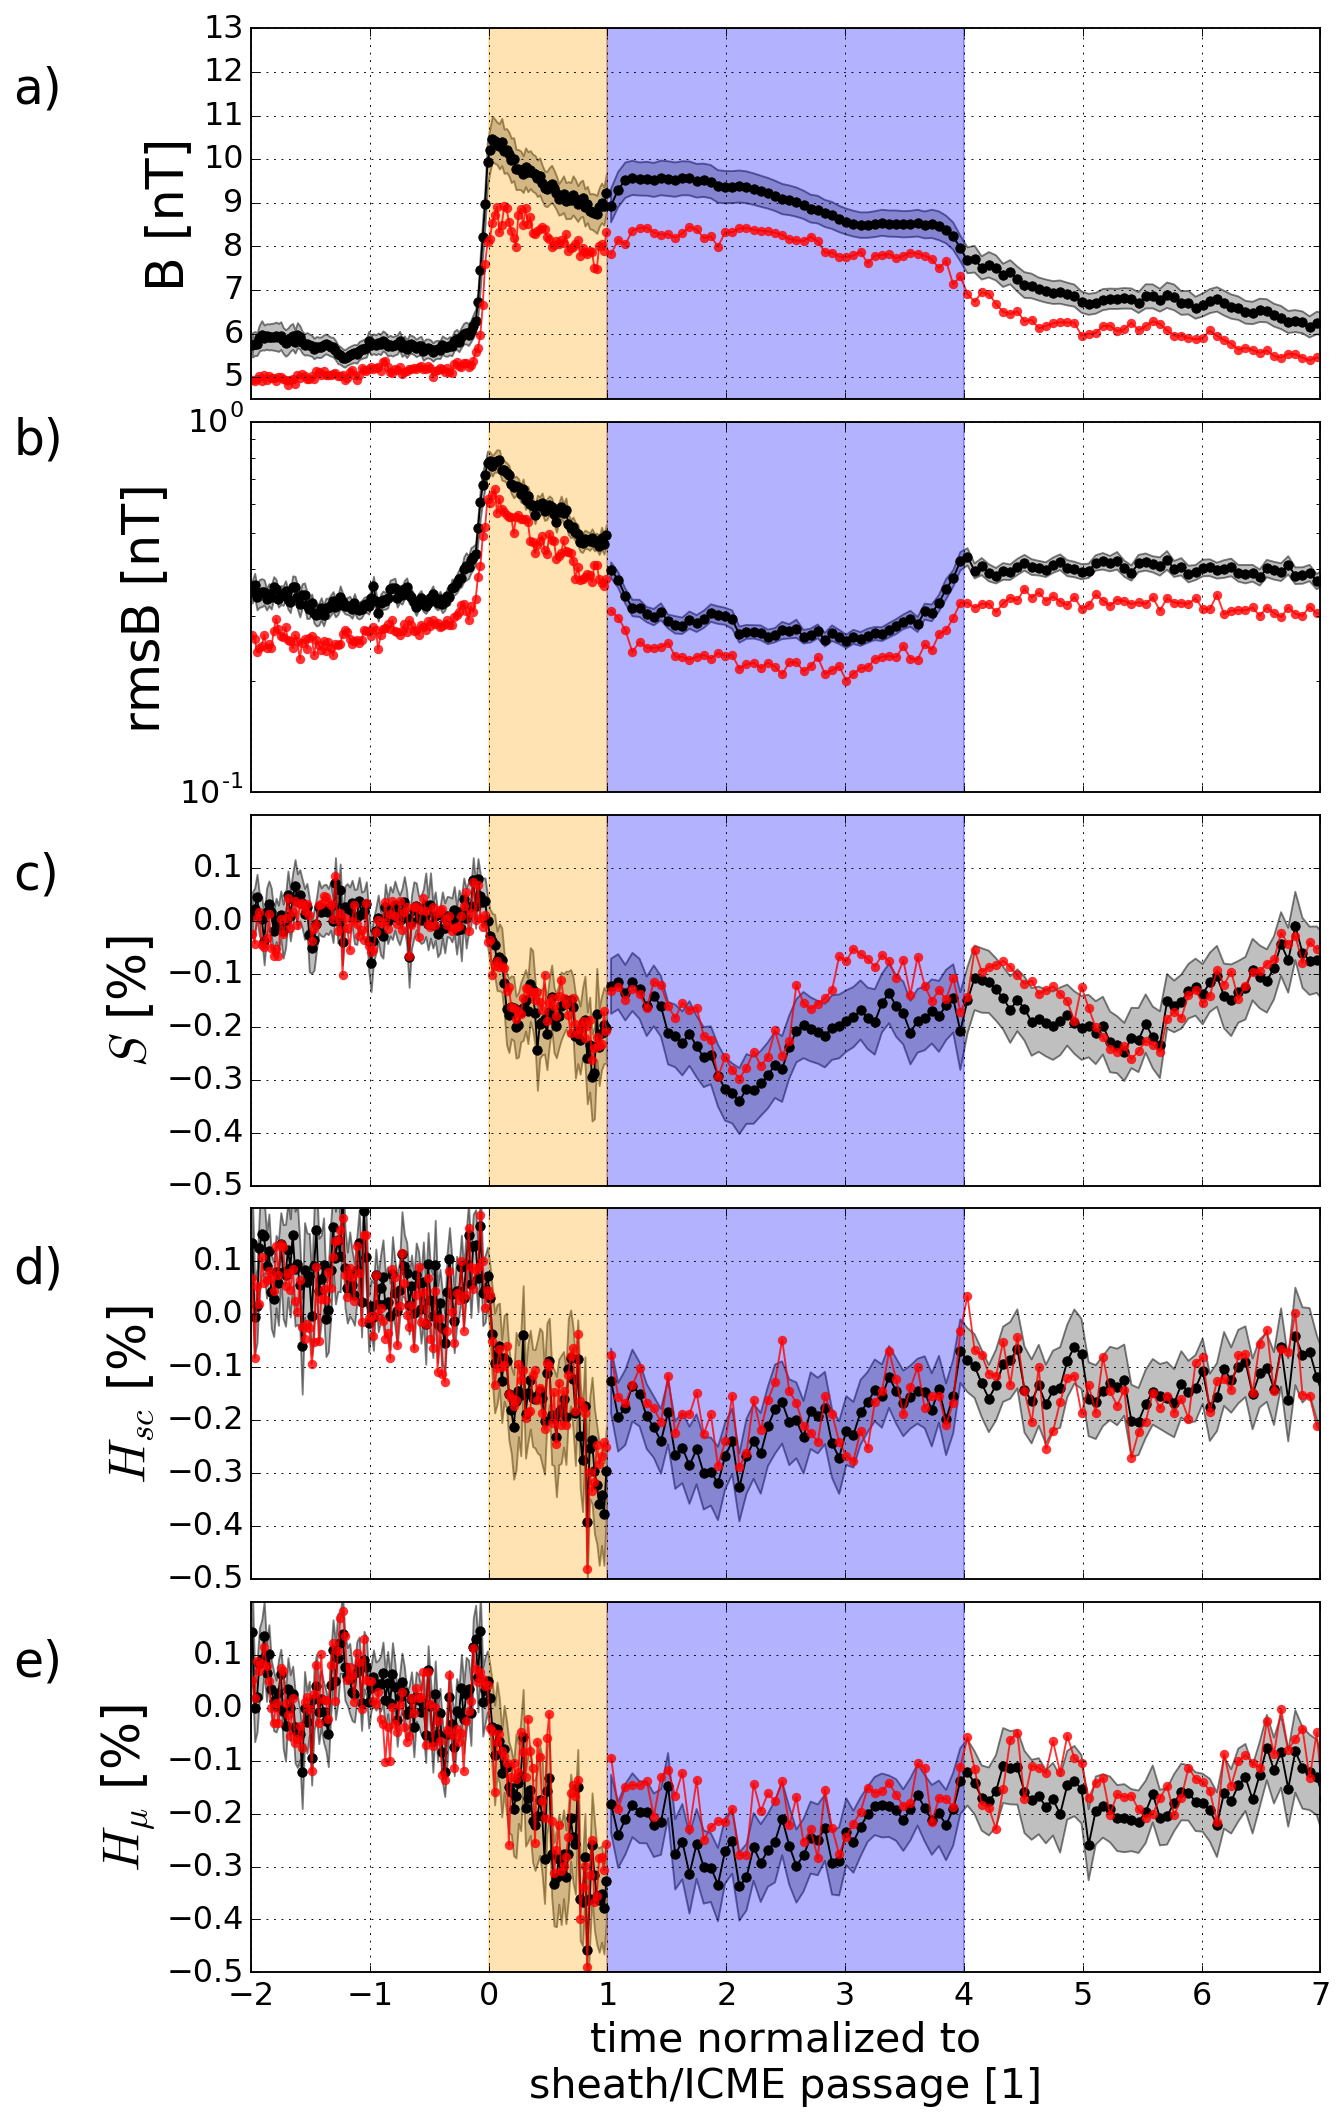
\includegraphics[width=0.7\linewidth]{Figs/ICME_scaler.png}
    \caption{Perfiles superpuestos de los flujos para diferentes energías en el observatorio Pierre Auger en los modos de detección histograma y scaler durante el paso de una ICME en el periodo de funcionamiento del observatorio: La gráfica \textit{a)} muestra un aumento en la magnitud del campo magnético interplanetario B, y la \textit{b)} muestra las fluctuaciones magnéticas rmsB que alcanzan su valor pico en el choque. La gráfica \textit{c)}, \textit{d)} y \textit{e)} muestran las desviaciones normalizadas del flujo de scaler, y las dos bandas de histograma.}
    \label{fig:ICME_scaler}
\end{figure}



\subsection{Efectos de la periodicidad solar en el fondo de RC medido}

%%%%%%%%%%%  FOURIER DE AUGER Y el NM que escogí
La anterior afirmación puede verse reflejada en la figura \ref{fig:CRIvsSN} donde se ilustra  las distribuciones y tendencias de SSN (Número de Manchas Solares), CRI (Íntensidad de Rayos Cósmicos) y SWS (Velocidad del Viento Solar). La resolución de cada una de estas series de tiempo es de 1 día, y en el caso de la tasa de scaler que es un indicador de la intensidad o flujo de rayos cósmicos secundarios, cuya resolución original es de 300s, hemos realizado un remuestreo a partir del promedio diario. Las tendencias se determinaron utilizando una media móvil de 15 días. Se observa una aparente anticorrelación entre el CRI y SSN. Las tendencias revelan claramente las variaciones a largo plazo en respuesta al SSN. El CRI muestra una periodicidad similar al ciclo solar de 11 años, mientras que el SSN muestra modulaciones irregulares en respuesta a las actividades solares. Sin embargo a simple vista no se observa a largo plazo una correlación con la velocidad del viento solar.

El comportamiento en el CRI podría deberse a la variabilidad de la amplitud del campo magnético heliosférico en el máximo solar, que reduce la afluencia de rayos cósmicos galácticos que entran en el sistema solar, y viceversa en el mínimo solar debido a la baja actividad magnética solar (\cite{Oloketuyi_2020}). Esto indica que el CRI es abundante fuera de la heliosfera, pero su influencia y modulaciones en la heliosfera dependen exclusivamente de las actividades solares.

\begin{figure}
    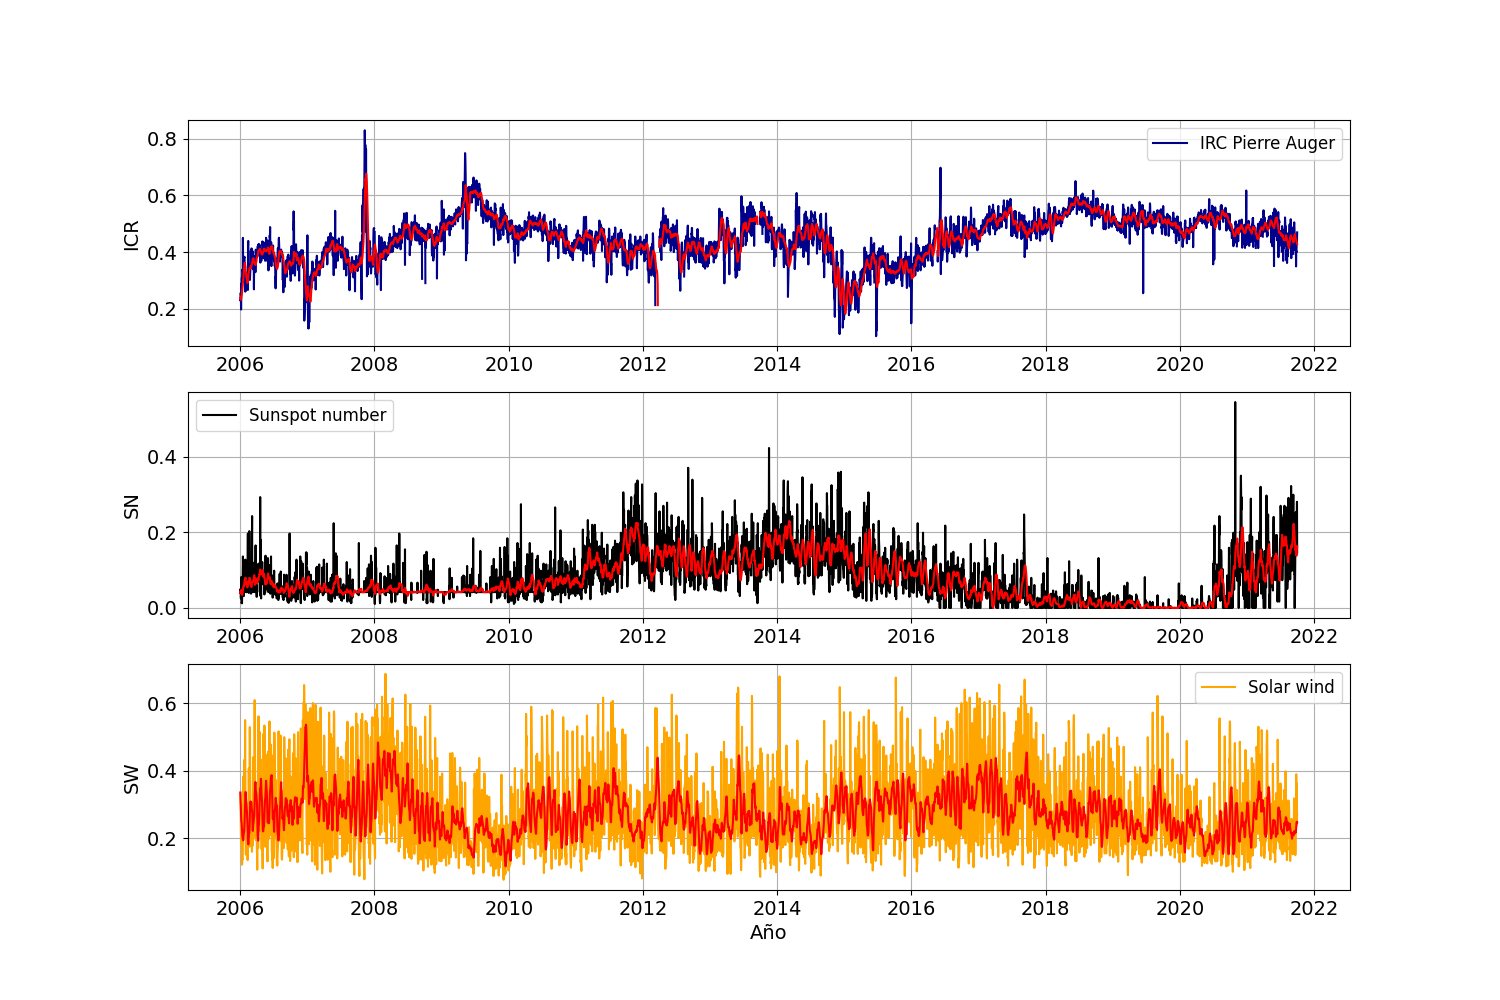
\includegraphics[width=1.1\linewidth]{Figs/Figr/CRI_SN_SW_over.png}
    \caption{Distribuciones y tendencias de SSN (Número de Manchas Solares), CRI (Intensidad de Rayos Cósmicos) y SWS (Velocidad del Viento Solar). Las tendencias se determinaron utilizando una media móvil de 90 días. Se observa una aparente anticorrelación entre el CRI y SSN. Eaboración propia.}
    \label{fig:CRIvsSN}
\end{figure}
Para verificar la aparente relación entre el CRI y las manchas solares, en la figura \ref{fig:sunspots_corr} se presenta los análisis de correlación cruzada entre el Número de Manchas Solares (SSN) diario y el Índice de Rayos Cósmicos (CRI) y la Velocidad del Viento Solar (SWS) (\cite{Oloketuyi_2020}) para los datos del Observatorio Pierre Auger y para las estaciones de neutrones Oulu y México. Se escogen estas dos estaciones debido a que Oulu sirve como referencia para la validación de los análisis respecto a otros trabajos, y méxico por su similitud en el valor de la rigidez de corte geomagnético.

%%%% correlación cruzada
Para calcular la correlación usaremos el método de correlación de Pearson, esta medida estadística evalúa la relación lineal entre dos variables continuas a partir de la obtención de un valor entre 0 y 1. Cuando el coeficiente es cercano a 1, indica una fuerte correlación positiva, es decir, cuando una variable aumenta, la otra también lo hace. Un coeficiente cercano a -1 indica una fuerte correlación negativa, lo que significa que cuando una variable aumenta, la otra disminuye:
$$ r_{xy} = \frac{\sum_{i=1}^{n} (x_i - \bar{x})(y_i - \bar{y})}{\sqrt{\sum_{i=1}^{n} (x_i - \bar{x})^2 \sum_{i=1}^{n} (y_i - \bar{y})^2}} $$
Donde:
- $x_i$ e $y_i$ son los valores individuales de las series $x$ e $y$ respectivamente.
- $\bar{x}$ y $\bar{y}$ son los promedios de las series $x$ e $y$ respectivamente.
- $n$ es el número de observaciones en cada serie.

Este coeficientes es actualmente una medida estándar en estadística porque es de fácil interpretación, y se ha usado en trabajos anteriores de fondo de rayos cósmicos (\cite{Usoskin_2005}, \cite{Oloketuyi_2020},\cite{Mendonça_2019},\cite{Davies_2023}).

%%% MEJORAR ESTA PARTE CON LA GRÁFICA DE SOLAR WIND
%%%%%
%%%%%%%%%
%%%%%%%%%%%%%%

El eje x de cada gráfico representa el desfase temporal en relación con el SSN y SW. El signo indica desplazamientos hacia adelante y hacia atrás, y el valor cero corresponde a la ausencia de desfase. Se observa que el CRI muestra una fuerte correlación negativa con el SSN para el ciclo solar 24, pero no se observa correlación significativa con el viento solar. Los picos positivos con valores de 0.38 y 0.57 se ajustan a una correlación positiva en $\approx$5 años, y los tres picos negativos, corresponden a una anticorrelación de 0.55 y 0.58 para un periodo de $\approx$ 8 a 9 años.
%Arreglar para tener la gráfica de correlación con el viento solar.
%Hacer la gráfica comparando el mismo intervalo de tiempo con la estación de neutrones Oulu y México
\begin{figure}
\centering
    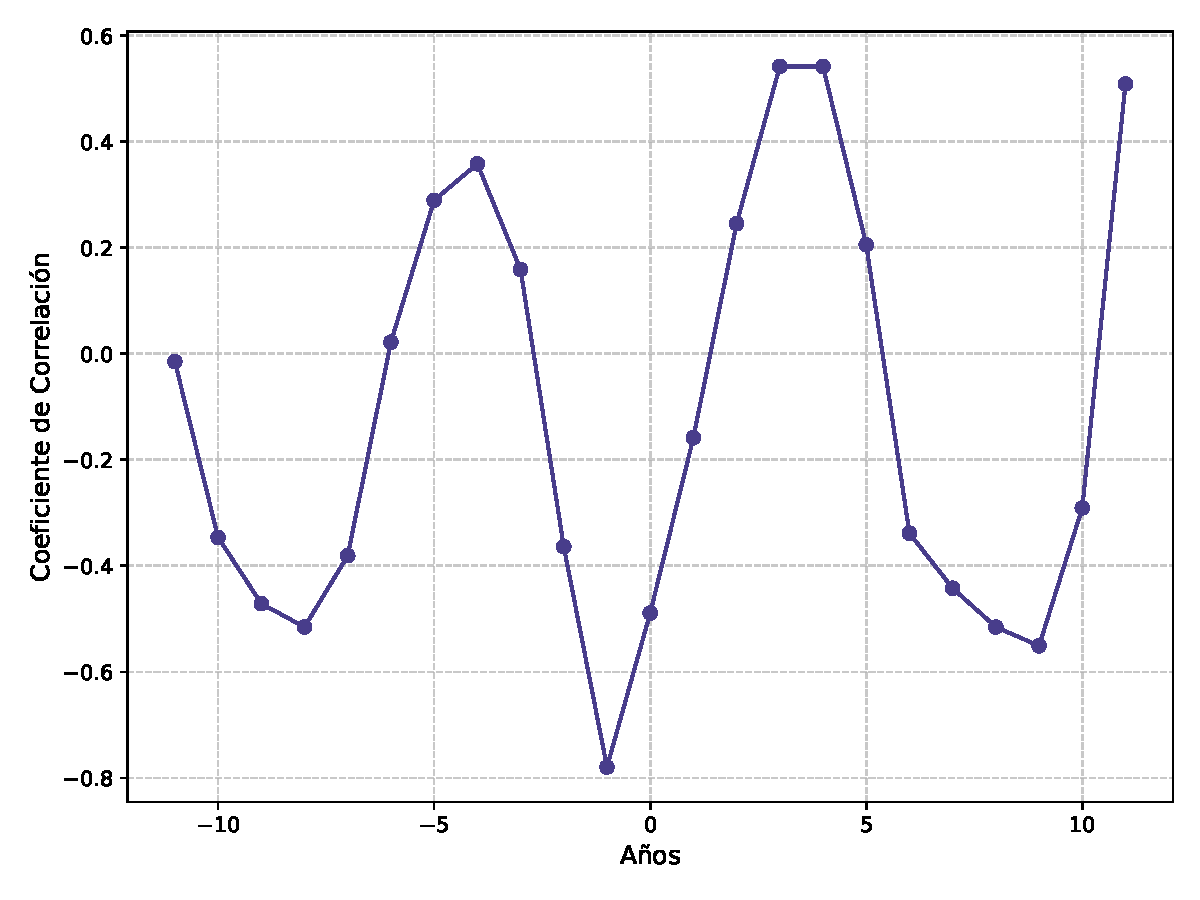
\includegraphics[width=0.7\linewidth]{Figs/Figr/CRI_SN_crosscorr.pdf}
    \caption{Análisis de correlación cruzada entre el Número de Manchas Solares (SSN) diario y el Índice de Rayos Cósmicos (CRI) y la Velocidad del Viento Solar (SWS) diarios usando el análisis de correlación cruzada usado en (\cite{Oloketuyi_2020}). El eje x de cada gráfico representa el desfase temporal en relación con el SSN. Los valores negativos indican desplazamientos hacia atrás, mientras que los positivos indican lo contrario, y el valor cero corresponde a la ausencia de desfase. Se observa que el CRI muestra una fuerte correlación negativa con el SSN para el ciclo solar 24. Elaboración propia}
    \label{fig:sunspots_corr}
\end{figure}
Es posible cuantificar entonces la sensibilidad del observatorio ante el ciclo solar 24, pero la escala que estamos utilizando nos impide ver los posibles efectos de las otras periodicidades en los datos por ejemplo, $( \thicksim 1, \thicksim13.5,\thicksim27, \thicksim186, \thicksim365$ d). Esto es posible mediante un análisis espectral. Para este trabajo usaremos el método de Blackman-Tukey (\cite{blackman}) aplicado en (\cite{noelia_2023}). El método de Blackman-Tukey es un poderoso enfoque no paramétrico para estimar la \textit{densidad espectral de potencia (PDS)} de series temporales. Éste método produce más del doble de estimaciones de la densidad espectral que la técnica FFT, por lo que las estimaciones B-T tienen una mayor resolución para el mismo coeficiente de variación (\cite{edge_1970}). 

%Este método se basa en el teorema de Wiener-Khinchin, que establece que se puede obtener el espectro de potencia de una serie de tiempo calculando primero su función de autocorrelación y luego aplicando la transformada de Fourier a la función de autocorrelación.

\textbf{Densidad espectral de potencia (PSD):}

La PSD es la medida que especifica los niveles de potencia de los componentes de frecuencia presentes en una señal, así se puede determinar el rango de potencia sobre el cual las frecuencias de la señal están operando. A partir del teorema de Wiener-Khinchin, se define como la transformada de Fourier de la la función de autocorrelación de una señal. Cuando se presenta un proceso aleatorio, la transformada de Fourier no puede ser aplicada directamente debido a que la mayoría de las realizaciones tienen formas irregulares y no pueden presentarse analíticamente (\cite{HerreraSepulveda_2017}). En estos casos solución para este inconveniente es entonces la aplicación de la función de autocorrelación . Esta función se define como el valor esperado de las variables aleatorias del proceso en los instantes de tiempo $t_1$ y $t_2$:
\begin{equation}
    R_{xx}(t_1 t_2) = E{X(t_1)X(t_2)}
\end{equation}
Si el proceso aleatorio es estacionario, la función de autocorrelación solo depende de la diferencia de los tiempos $(\tau)$:
\begin{equation}
    R_{xx}(\tau) = E{X(t)X(t+\tau)}
\end{equation}
Ahora bien, la densidad espectral de potencia PSD está dada por:
\begin{equation}
   S_{xx}(\omega) = \int_{-\infty}^{\infty} R_{xx}(\tau) e^{-j\omega\tau} d\tau
\end{equation}
Existen dos técnicas principales para estimar la Densidad Espectral de Potencia (DEP): el método paramétrico y el no paramétrico. El método paramétrico utiliza un modelo para el proceso aleatorio para estimar el espectro de potencia, incluyendo técnicas como el modelo de media móvil (MA), el modelo autoregresivo (AR) y el modelo autoregresivo de media móvil (ARMA). Por otro lado, el método no paramétrico estima primero la secuencia de autocorrelación de un conjunto de datos y luego estima el espectro de potencia a través de la Transformada de Fourier de la secuencia de autocorrelación estimada, utilizando técnicas como el periodograma, el método de Barlett, el método de Welch y el método de Blackman-Tukey (\cite{HerreraSepulveda_2017}).



\begin{comment}
    Suponiendo que tras las correcciones por presión y temperatura no haya más variables atmosféricas que afecten a la tasa de recuento, un análisis espectral proporcionará periodicidades relacionadas con los efectos heliosféricos. Existen varias técnicas para realizar una estimación de la densidad espectral de potencia (PDS). Entre los métodos no paramétricos se encuentra el método de Blackman-Tukey (Blackman & Tukey, 1958). Este método se basa en el hecho de que la transformada de Fourier de una función de autocorrelación de una serie temporal es equivalente a su espectro de potencia. Ponderar la función de autocorrelación según diversas formas es un método tradicional para reducir una fuga de potencia. Estimamos la PSD de la S 00 horaria aplicando el método de Blackman-Tukey y considerando la ventana de Hanning de un tamaño igual a 0,3 de la longitud de los datos. Para determinar la importancia de los picos espectrales, se ha empleado la generación de un espectro de ruido rojo. Los picos espectrales que tienen amplitudes superiores al intervalo de confianza del 95 % se distinguen estadísticamente del espectro de ruido rojo de fondo.
\end{comment}

La gráfica \ref{FFT} Muestra la expansión discreta en serie de Fourier de las tasas escalares observadas en escala logarítmica. Los picos más agudos en la potencia espectral son visibles para una señal con una frecuencia de un día solar. Esta señal diurna es debida a la rotación de la Tierra en el viento solar magnetizado y ha sido observada con Auger anteriormente.

\begin{figure}
\centering
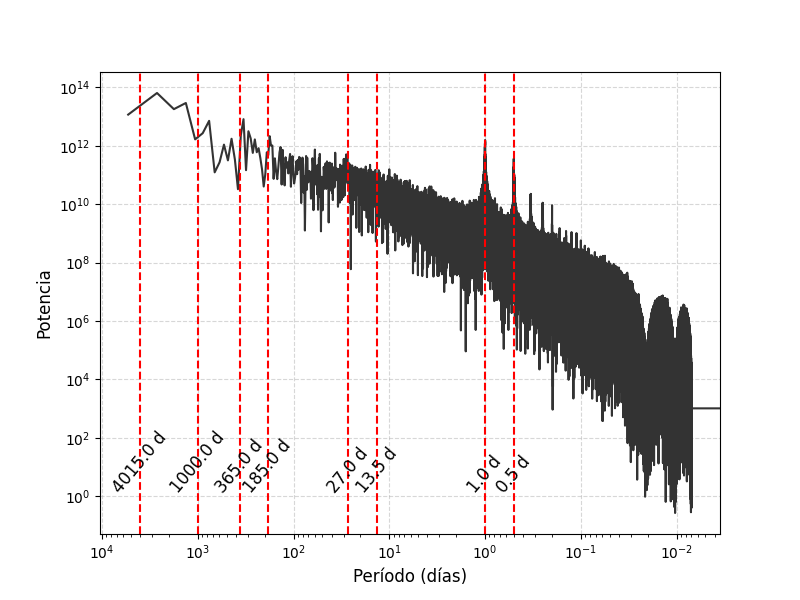
\includegraphics[width=0.8\linewidth]{Figs/Figr/fft_period.png}
    \caption{Pendiente modificar con Autocorrelación para eliminar el ruido.}
    \label{FFT}
\end{figure}




\subsection{Sensibilidad a eventos transitorios}
%%%%% BÚSQUEDA DE FORBUSH
La resolución temporal de la tasa de scaler de 300s puede utilizarse para la búsqueda de eventos transitorios como los Forbush Decrease cuya presencia en los datos del Observatorio ya ha sido reportada. El presente trabajo no busca identificar los eventos, sino caracterizar la sensibilidad del Observatorio ante FE (Eventos Forbush) de diferentes intensidades. Para ello, vamos a usar la información del catálogo de eventos Forbush y disturbios interplanetarios como se describe en la sección 3.1, en los periodos 2006 -2019 estableciendo criterios físicos para la selección de eventos significativos. La gráfica \ref{fig:FD_events} muestra todas las magnitudes de los FE registrados en la base de datos, clasificados por la fuente que lo ha generado. Se observa que la mayor cantidad de eventos son aquellos que no tienen una relación confirmada  con fenómenos solares transitorios (puntos azules). No obstante, estos FE tienen en su mayoría magnitudes muy bajas y no presentan un comportamiento fuertemente ligado al ciclo solar, como sí se observa en los eventos asociados a Ondas de Choque Interplanetario OCI y comienzos de tormentas súbitas SSC. Especialmente estos eventos son los que presentan una mayor magnitud.
\begin{figure}
\centering
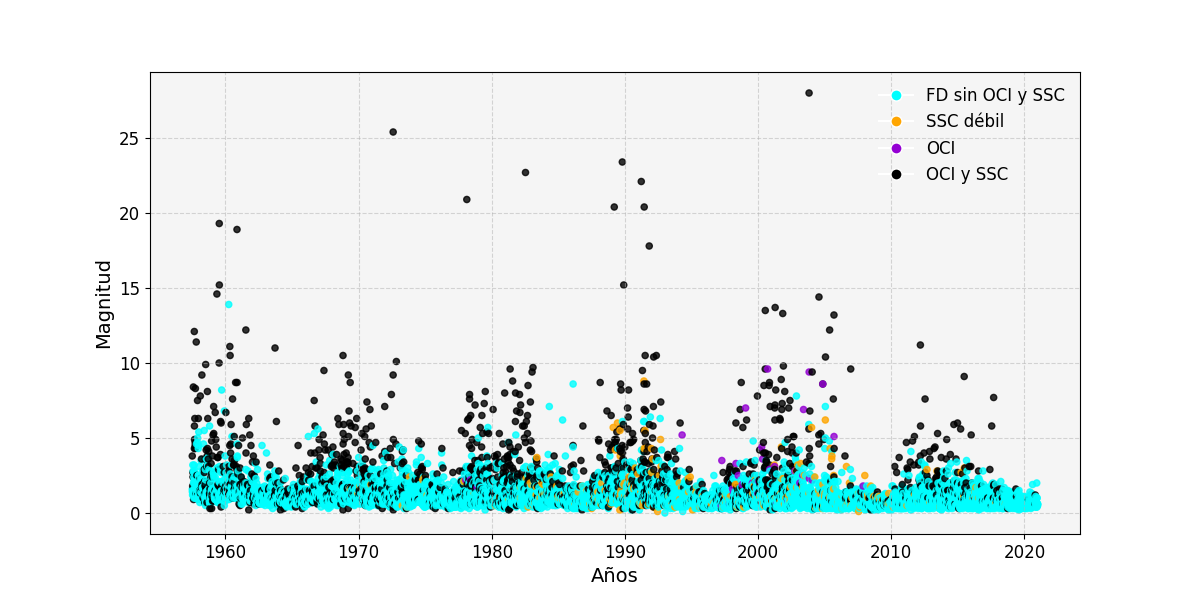
\includegraphics[width=1.2\linewidth]{Figs/Figr/forbush_events.png}
    \caption{Magnitudes de los FE registrados en la base de datos, clasificados por la fuente que lo ha generado. }
    \label{fig:FD_events}
\end{figure}
Se seleccionaron los FE que cumplieran con las siguientes características en la base de datos:
\begin{itemize}
    \item Eventos cuyas fuentes son Ondas de Choque Interplanetarias OCI y Comienzos de tormenta súbita SSC (OType = 1).
    \item Alta confiabilidad en la asociación del FE con la fuente (Qs = 4 y 5).
\end{itemize}
En total son 148 FE que cumplen con estas características para el periodo de tiempo de funcionamiento del observatorio, la tabla (\ref{tabla_FE_Auger}) muestra la lista de eventos seleccionados con algunos parámetros de interés como la fecha y hora del evento solar con el que está asociado, el tipo de fuente y la magnitud.



%%%%%%%%%%%%%%%%   TABLAAAAAAAAAAAA FORBUSHHHH

%%%%%%%%%%%%%%%%

La gráfica \ref{hist_FE} muestra el histograma de magnitudes para los FE en donde se observa que la mayor cantidad de eventos tiene magnitud por debajo de dos (en total el $60.14\%$). Revisemos ahora la ventana correspondiente al ciclo solar 24 y contrastemos la ocurrencia de FEs con la tasa de scaler. La gráfica \ref{fig:FD_scaler} muestra la magnitud normalizada de FD entre 2006 a 2021 a la vez junto con la tasa de scaler normalizada. La barra de color en la parte superior divide el eje x en 15 secciones correspondiente a cada año  y el color representa la candidad de DF registrados en cada año.

Se observa  que la mayor cantidad de FD $55.41\%$ se encuentran en la zona de máxima actividad solar (2012-2015) en esta región, en esta región se encuentra el $71.20\%$ de los eventos con magnitud >2 en todo el periodo de registro del observatorio.
\begin{figure}
    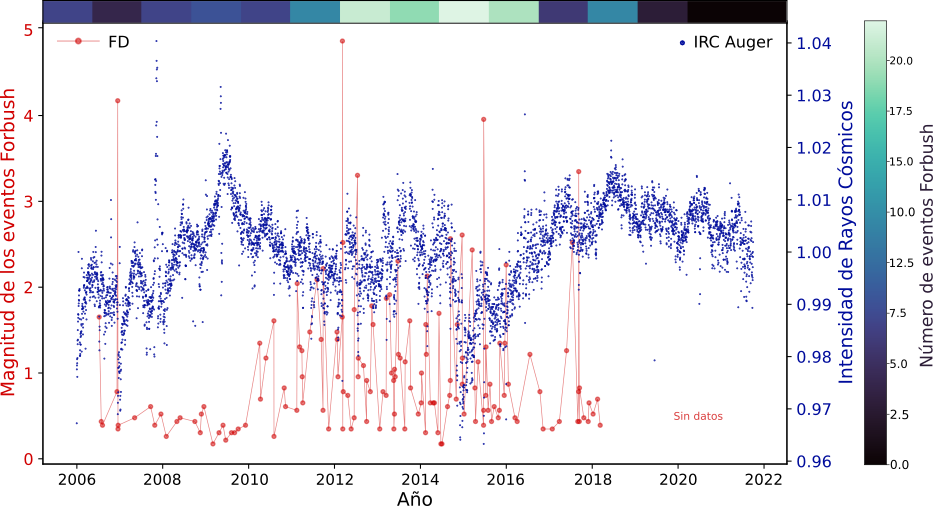
\includegraphics[width=1\linewidth]{Figs/Figr/FD_Scaler_AUGER.png}
    \caption{Enter Caption}
    \label{fig:FD_scaler}
\end{figure}
%ESTO VA ARRIBA EN LA PERIODICIDAD DIARIA
%En el trabajo de \cite{martin_ICRC} realizado también para el Observatorio Pierre Auger se reporta un comportamiento
Lo anterior confirma la hipotesis que asocia las irregularidades en los perfiles de scaler diarios en el periodo de tiempo de máxima actividad solar con una mayor tasa de FE.

Veamos cómo se comportan los scaler a cortas escalas, en el rango de la duración habitual de un FE (
días). El flujo de fondo de RC es muy sensible a fluctuaciones de diferentes frecuencias causadas por la actividad solar y esto supone un desafío a la hora de aplicar técnicas de filtrado que elimine ruido. Identificar eventos transitorios implica caracterizar muy bien el background de la señal medida por el observatorio. Sin embargo las técnicas de filtrado como la ventana móvil pueden ser útiles para sualizar la señar y hacer nuestra caracterización de forbush in situ. 

%ESCRIBIR TEORÍA DEL PROMEDIO MÓVIL

Con la figura \ref{FD1} podemos observar un Forbush con magnitud 9.5 medido por los scaler con la señal sin filtrar y con la señal filtrada. El suavizado para eliminar la priodicidad diaria se realiza con la ventana móvil de un día. ¿Cuál es entonces la mínima sensibilidad que tiene el observatorio a estos eventos?

%Para ello, vamos a remover periodicidad diaria de los datos que interfieren con la identificación de estos eventos


%%%%%%%%%% O HACEMOS UNA DONDE INTENTEMOS RESTAR LOS FORBUSH 
%%%%%%%%%%% SERÍA MUCHO RETO
%%%%%%%%%%%% CALCULAR LA AMPLITUD? NO SÉ

\section{Datos abiertos y ciencia ciudadana}